\documentclass[11pt]{article}
\usepackage{fullpage} % changes the margin
\usepackage{setspace}
\usepackage[pdftex]{graphicx}
\usepackage[
	pdfauthor={Brian Weinstein},
	pdftitle={Homework 1},
	bookmarks=true,
	colorlinks=true,
	linkcolor=blue,
	urlcolor=blue,
	citecolor=blue,
	pdftex,
	linktocpage=true
	]{hyperref}
\usepackage[textsize=tiny]{todonotes}
\usepackage{float}
\setlength\parindent{0pt}

%\usepackage{fancyhdr}
%\usepackage{amssymb}
%\pagestyle{fancy}
%\lhead{Homework 01}
%\chead{Brian Weinstein}
%\rhead{STAT S4240 002}



\begin{document}

\noindent
\large\textbf{STAT S4240 002, Homework 1} \hfill \textbf{Brian Weinstein}\\
\normalsize 13 July, 2015 \hfill  bmw2148\\


\section*{Problem 1: \href{http://www-bcf.usc.edu/~gareth/ISL/}{James} 2.4, Exercise 8}

\subsection*{Part a}

\begin{figure}[H]
	\centering
	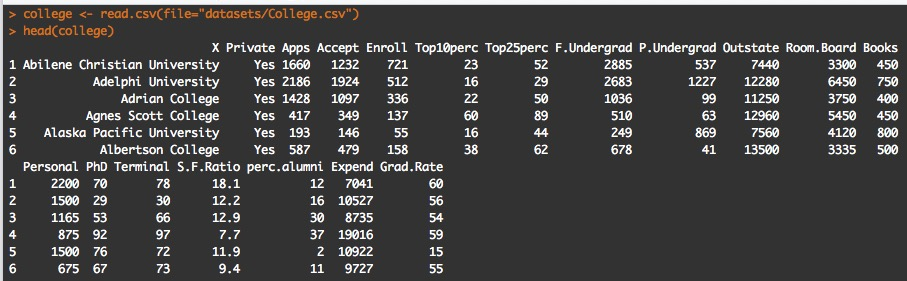
\includegraphics[width=6.5in]{8a.jpeg}
	%\caption{}
	%\label{fig:figName}
\end{figure}


\subsection*{Part b}

\begin{figure}[H]
	\centering
	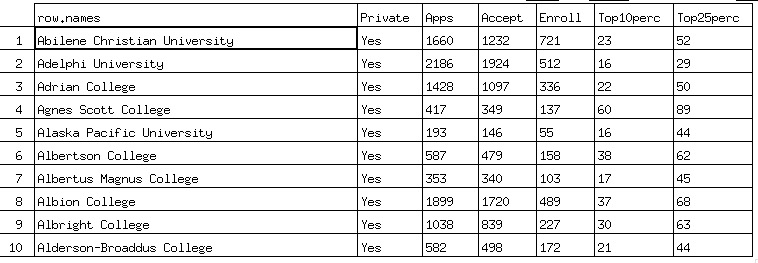
\includegraphics[width=6.5in]{8b.jpeg}
	%\caption{}
	%\label{fig:figName}
\end{figure}

\subsection*{Part c}

\subsubsection*{Part i}

\begin{figure}[H]
	\centering
	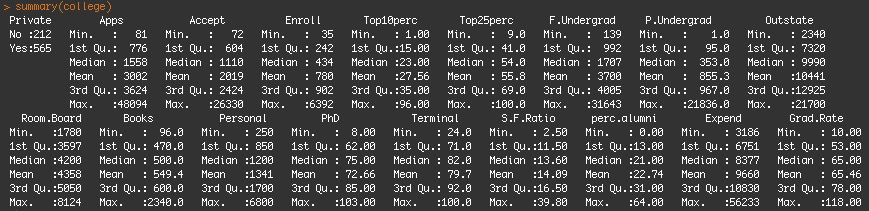
\includegraphics[width=6.5in]{8ci.jpeg}
	%\caption{}
	%\label{fig:figName}
\end{figure}

\subsubsection*{Part ii}

\begin{figure}[H]
	\centering
	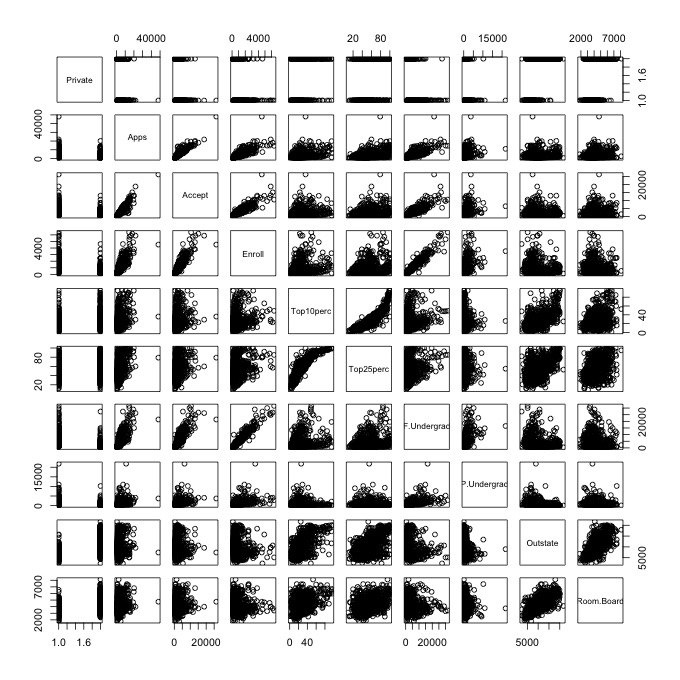
\includegraphics[width=5.5in]{8cii.jpeg}
	%\caption{}
	%\label{fig:figName}
\end{figure}

\subsubsection*{Part iii}

\begin{figure}[H]
	\centering
	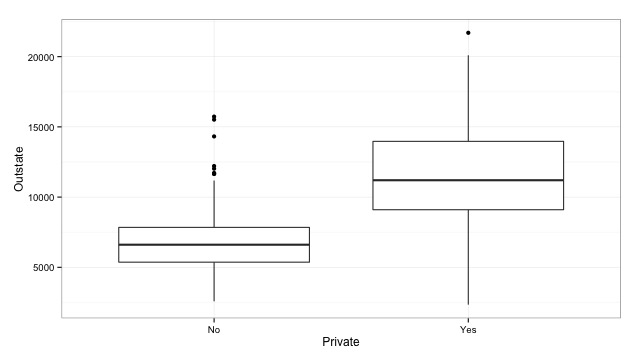
\includegraphics[width=6.5in]{8ciii.jpeg}
	%\caption{}
	%\label{fig:figName}
\end{figure}

\subsubsection*{Part iv}

There are 78 colleges categorized as "Elite".

\begin{figure}[H]
	\centering
	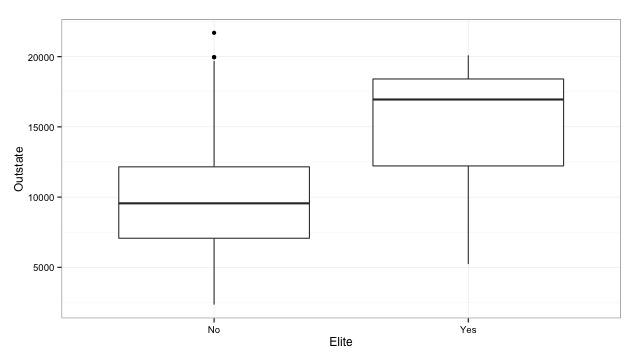
\includegraphics[width=6.5in]{8civ.jpeg}
	%\caption{}
	%\label{fig:figName}
\end{figure}

\subsubsection*{Part v}

\begin{figure}[H]
	\centering
	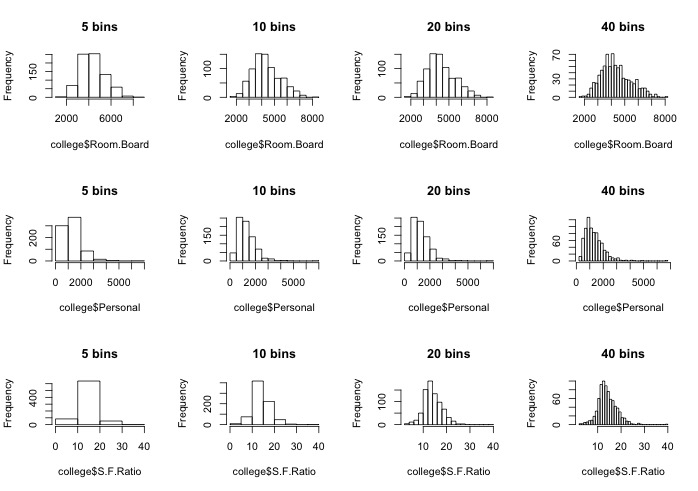
\includegraphics[width=6.5in]{8cv.jpeg}
	%\caption{}
	%\label{fig:figName}
\end{figure}

\subsubsection*{Part vi}

I chose to explore acceptance and enrollment rates, with acceptance rate defined as the number of students accepted per application received (\texttt{college\$Accept/college\$Apps}), and enrollment rate defined as the number of students enrolled per applicant accepted (\texttt{college\$Enroll/college\$Accept}).

\begin{figure}[H]
	\centering
	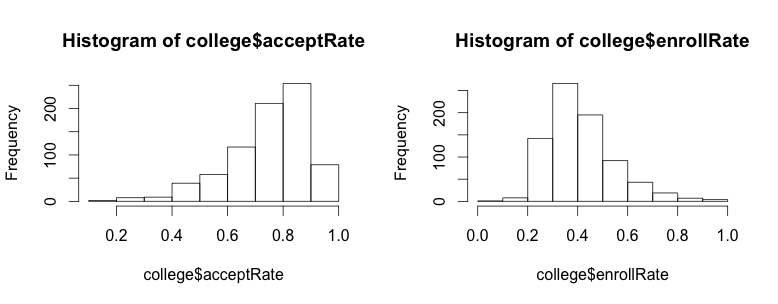
\includegraphics[width=5.5in]{8cvi_histograms.png}
	%\caption{}
	%\label{fig:figName}
\end{figure}

Somewhat surprisingly, there's little correlation between acceptance and enrollment rate.
\begin{verbatim}
> cor(college$acceptRate, college$enrollRate)
[1] 0.0824304
\end{verbatim}

\begin{figure}[H]
	\centering
	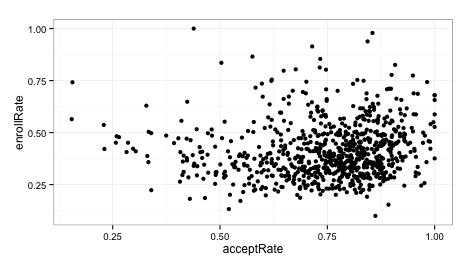
\includegraphics[width=5.5in]{8cvi_enroll_vs_accept.png}
	%\caption{}
	%\label{fig:figName}
\end{figure}


I also looked at summary statistics by public vs private schools.
\begin{verbatim}
> college %>%
+   group_by(Private) %>%
+   summarize(min.acceptRate=min(acceptRate),
+             median.acceptRate=median(acceptRate),
+             mean.acceptRate=mean(acceptRate),
+             max.acceptRate=max(acceptRate),
+             min.enrollRate=min(enrollRate),
+             median.enrollRate=median(enrollRate),
+             mean.enrollRate=mean(enrollRate),
+             max.enrollRate=max(enrollRate)) %>%
+   as.data.frame()


  Private min.acceptRate median.acceptRate mean.acceptRate max.acceptRate min.enrollRate
1      No      0.3397060         0.7443387       0.7265305              1     0.13242009
2     Yes      0.1544863         0.7885653       0.7545812              1     0.09975397
  median.enrollRate mean.enrollRate max.enrollRate
1         0.4405908       0.4620216      0.9382716
2         0.3660934       0.3932510      1.0000000
\end{verbatim}



\begin{figure}[H]
	\centering
	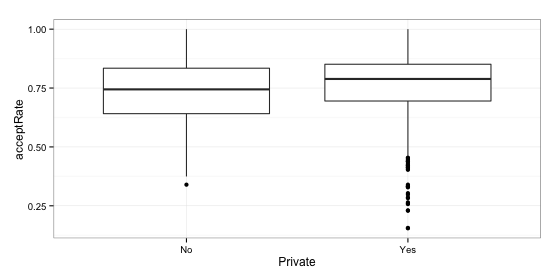
\includegraphics[width=5.5in]{8cvi_acceptRate_boxplots.png}
	%\caption{}
	%\label{fig:figName}
\end{figure}

\begin{figure}[H]
	\centering
	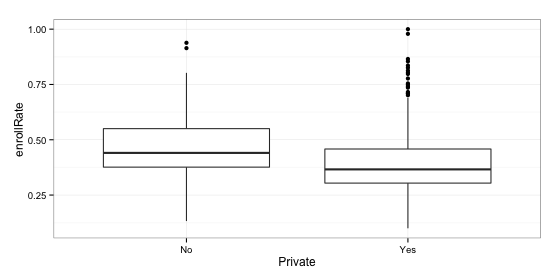
\includegraphics[width=5.5in]{8cvi_enrollRate_boxplots.png}
	%\caption{}
	%\label{fig:figName}
\end{figure}



\section*{Problem 2: \href{http://www-bcf.usc.edu/~gareth/ISL/}{James} 2.4, Exercise 9}

\subsection*{Part a}
Quantitative predictors: \texttt{mpg}, \texttt{cylinders}, \texttt{displacement}, \texttt{horsepower}, \texttt{weight}, \texttt{acceleration}, \texttt{year}\\
Qualitative predictors: \texttt{origin}, \texttt{name}

\subsection*{Part b}
\begin{verbatim}
  statistic  mpg cylinders displacement horsepower weight acceleration year origin name
1       min  9.0         3           68         46   1613          8.0   70     NA   NA
2       max 46.6         8          455        230   5140         24.8   82     NA   NA
\end{verbatim}

\subsection*{Part c}

\begin{verbatim}
  statistic       mpg cylinders displacement horsepower    weight acceleration      year origin name
1      mean 23.445918  5.471939      194.412  104.46939 2977.5842    15.541327 75.979592     NA   NA
2        sd  7.805007  1.705783      104.644   38.49116  849.4026     2.758864  3.683737     NA   NA
\end{verbatim}

\subsection*{Part d}

\begin{verbatim}
  statistic       mpg cylinders displacement horsepower    weight acceleration      year origin name
1       min 11.000000  3.000000     68.00000   46.00000 1649.0000     8.500000 70.000000     NA   NA
2       max 46.600000  8.000000    455.00000  230.00000 4997.0000    24.800000 82.000000     NA   NA
3      mean 24.404430  5.373418    187.24051  100.72152 2935.9715    15.726899 77.145570     NA   NA
4        sd  7.867283  1.654179     99.67837   35.70885  811.3002     2.693721  3.106217     NA   NA
\end{verbatim}

\subsection*{Part e}


MPG generally increased between 1970 and 1982.
\begin{figure}[H]
	\centering
	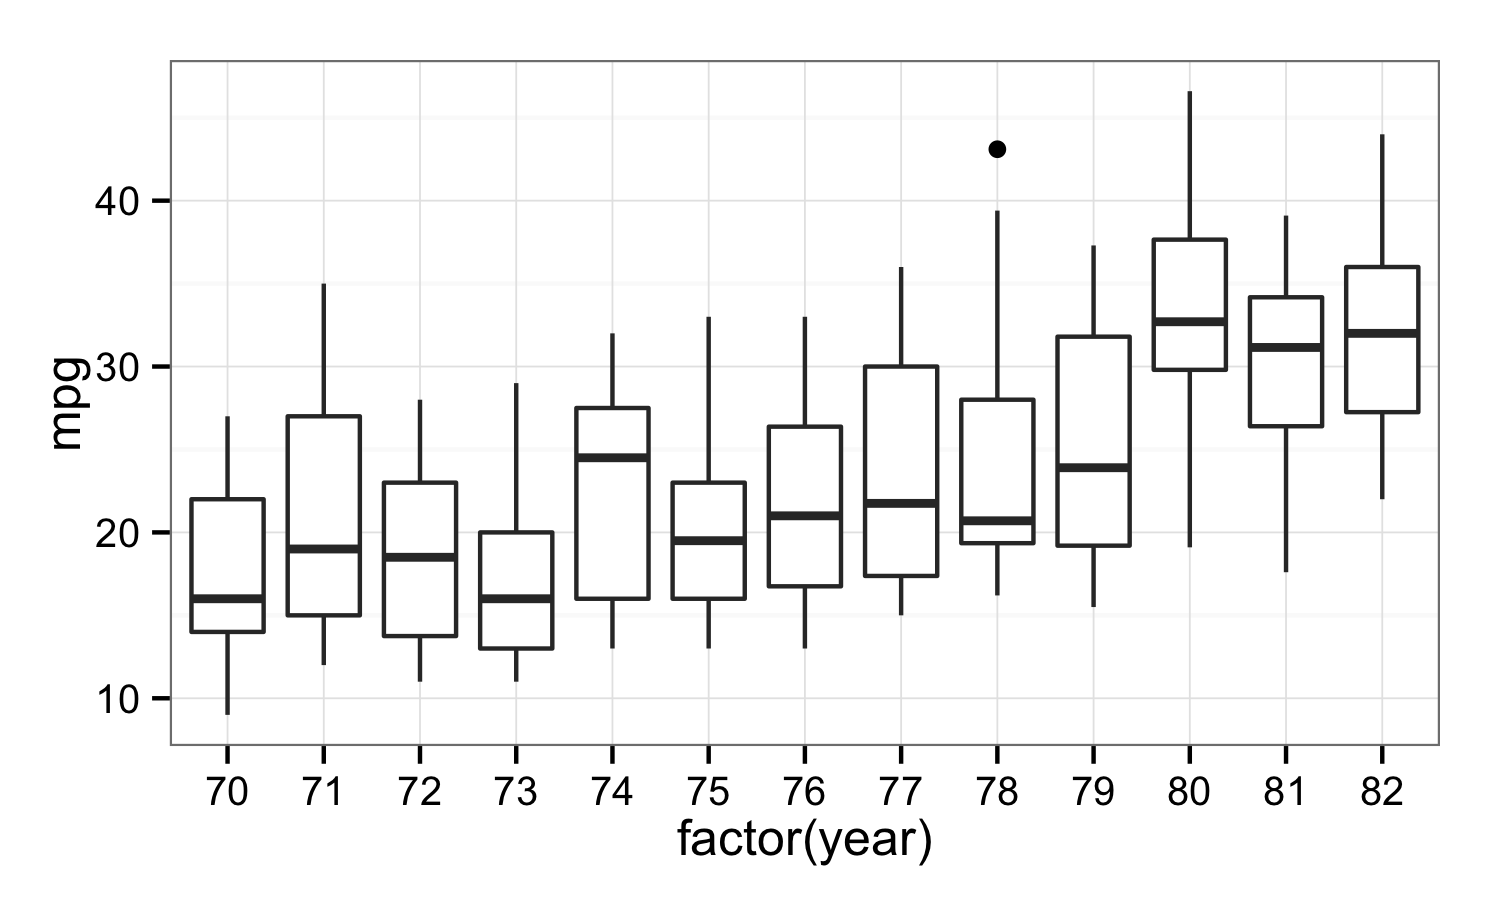
\includegraphics[width=5in]{9e_mpg_vs_year.png}
	\caption{MPG vs year}
	\label{fig:mpg_vs_year}
\end{figure}

As the number of cylinders increases, MPG generally decreases.\begin{figure}[H]
	\centering
	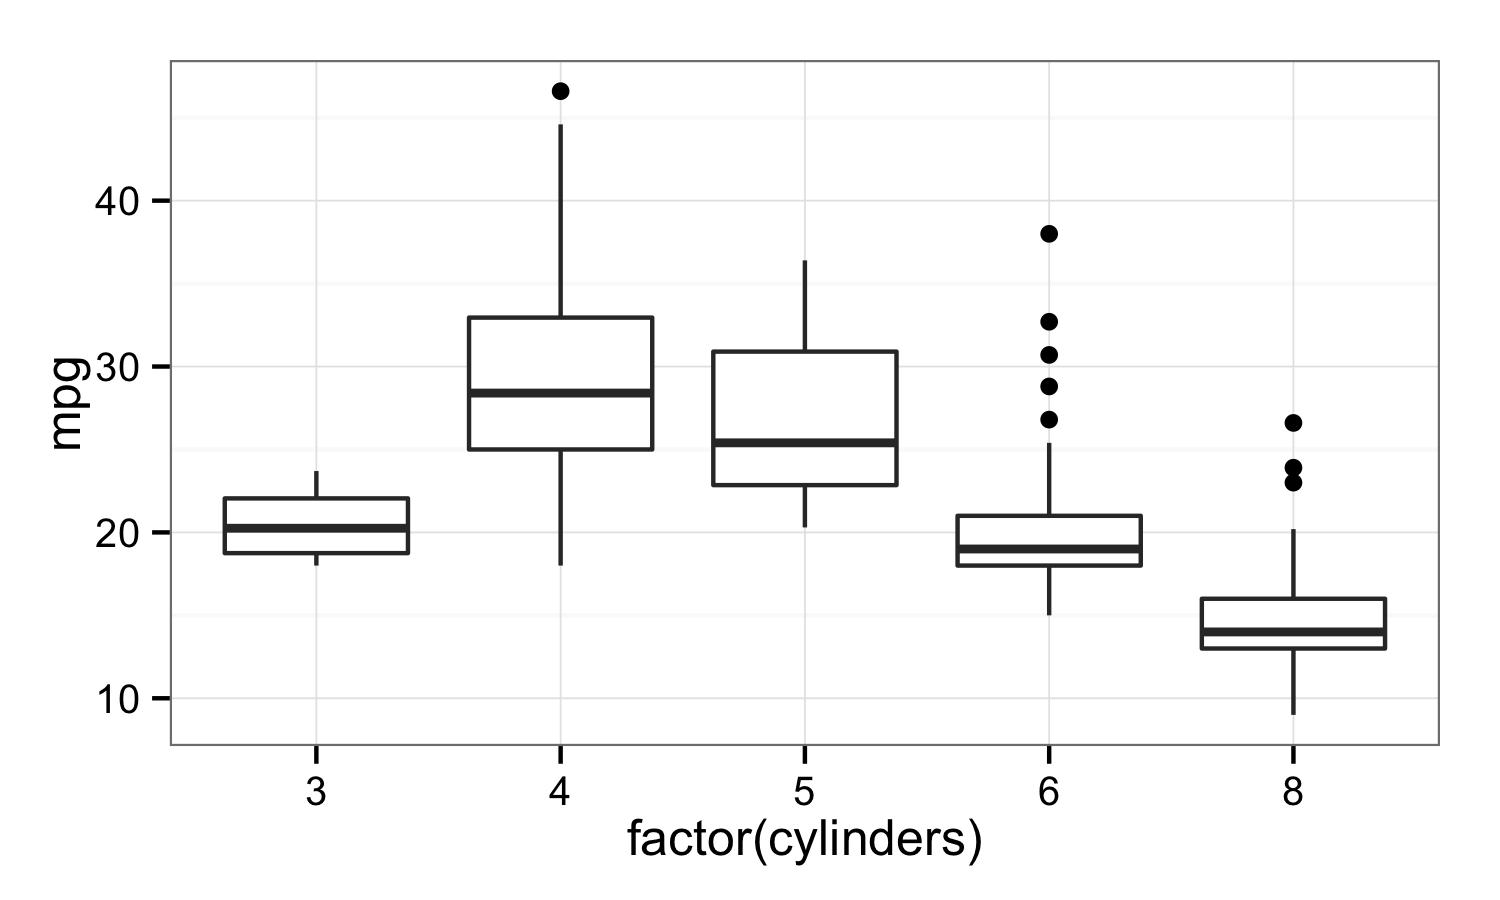
\includegraphics[width=5in]{9e_mpg_by_cyl.png}
	\caption{MPG vs number of cylinders}
	\label{fig:mpg_vs_cyl}
\end{figure}


There isn't a particularly strong relationship between weight and acceleration (at least not one that is easily seen graphically).
\begin{figure}[H]
	\centering
	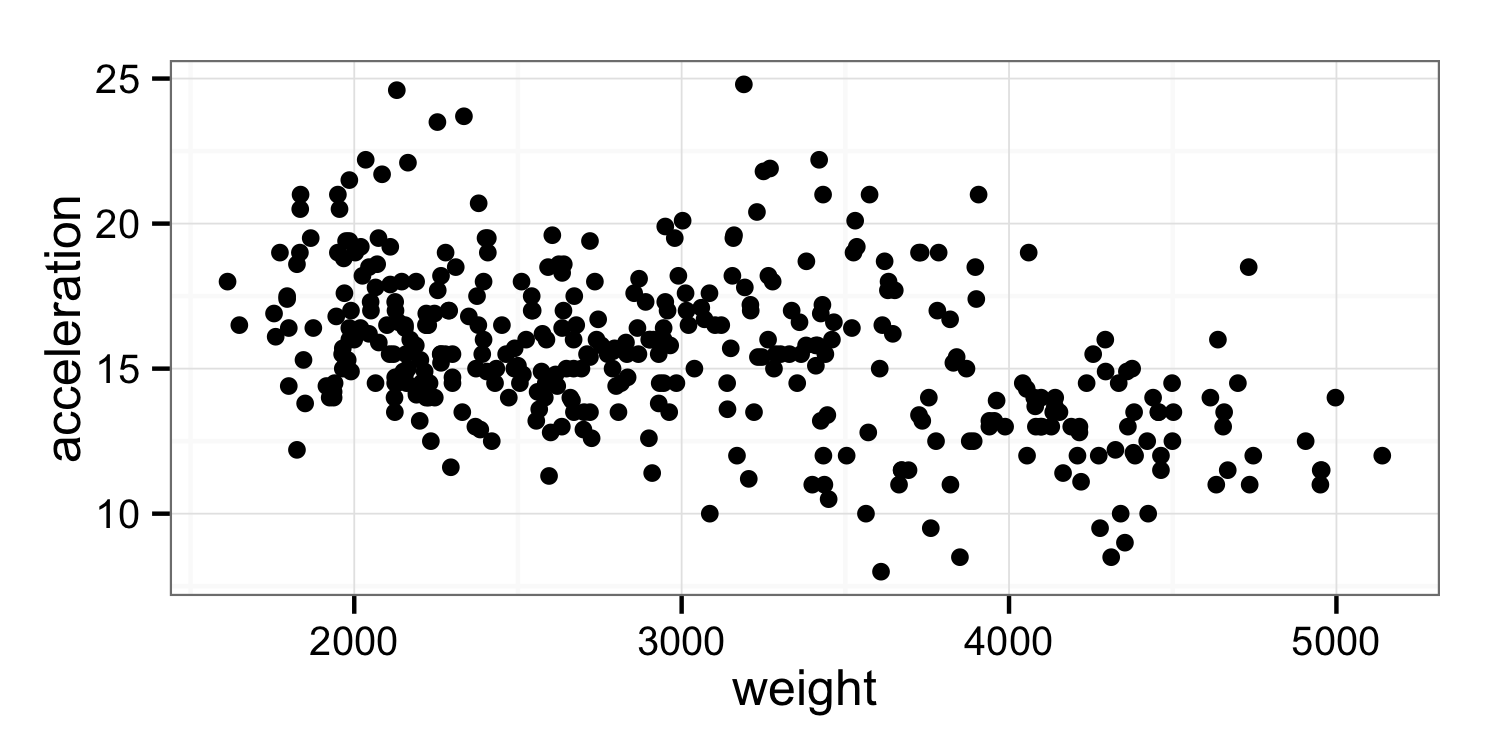
\includegraphics[width=5in]{9e_acc_vs_weight.png}
	%\caption{}
	%\label{fig:figName}
\end{figure}


But there is a strong negative relationship between horsepower and acceleration.
\begin{figure}[H]
	\centering
	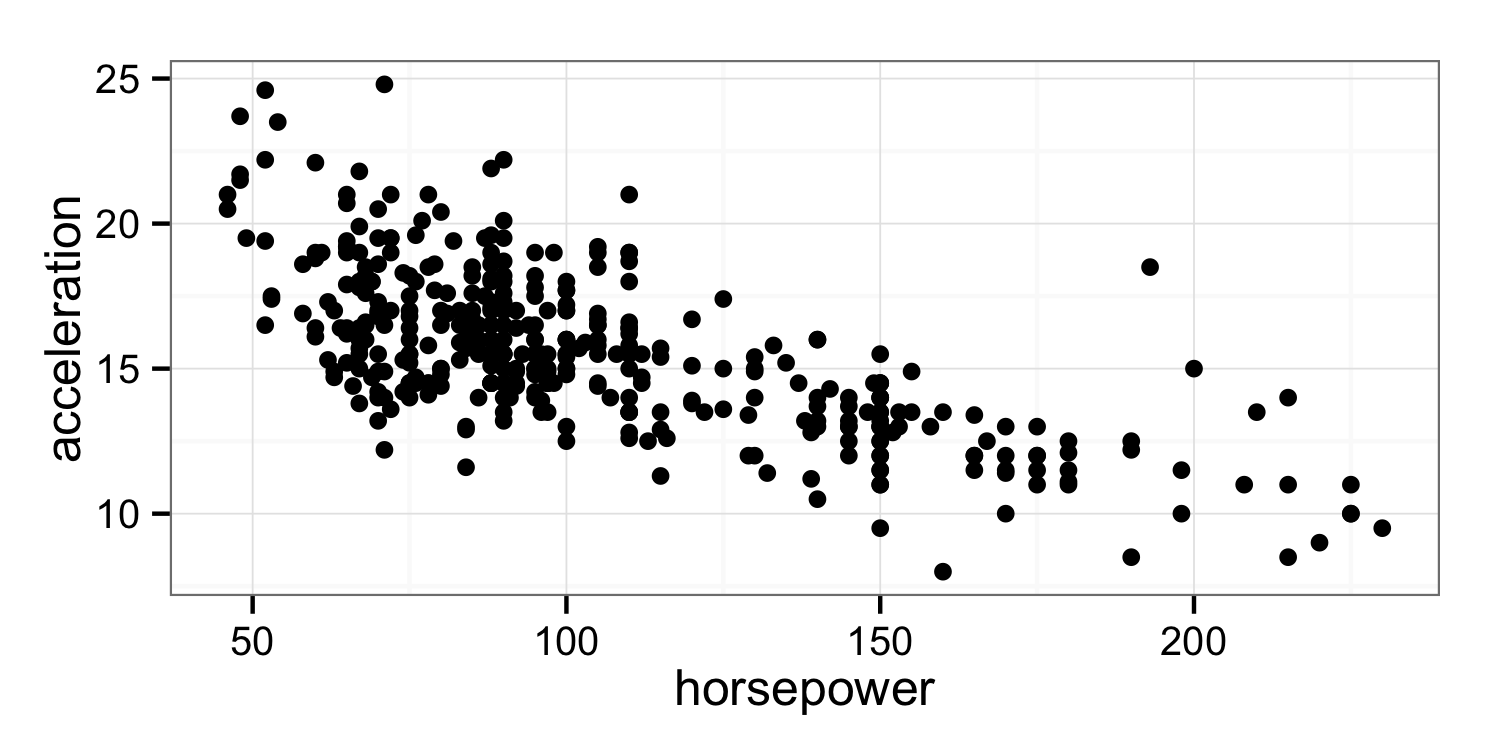
\includegraphics[width=5in]{9e_acc_vs_hp.png}
	%\caption{}
	%\label{fig:figName}
\end{figure}

And unsurprisingly, as the weight of a car increases, so does its horsepower.
\begin{figure}[H]
	\centering
	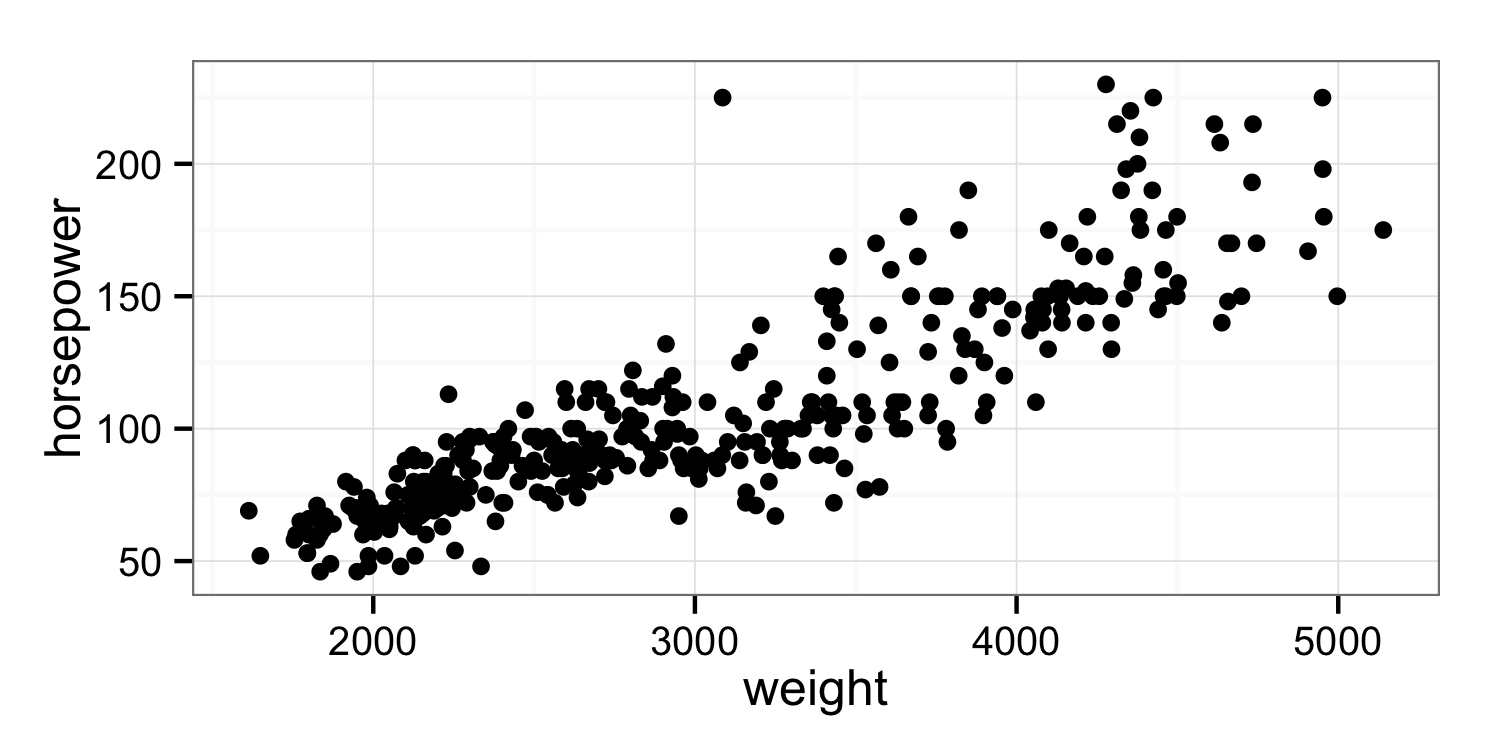
\includegraphics[width=5in]{9e_hp_vs_weight.png}
	%\caption{}
	%\label{fig:figName}
\end{figure}


Japanese cars (3) are usually lighter than American (1) and European (2) cars.
\begin{figure}[H]
	\centering
	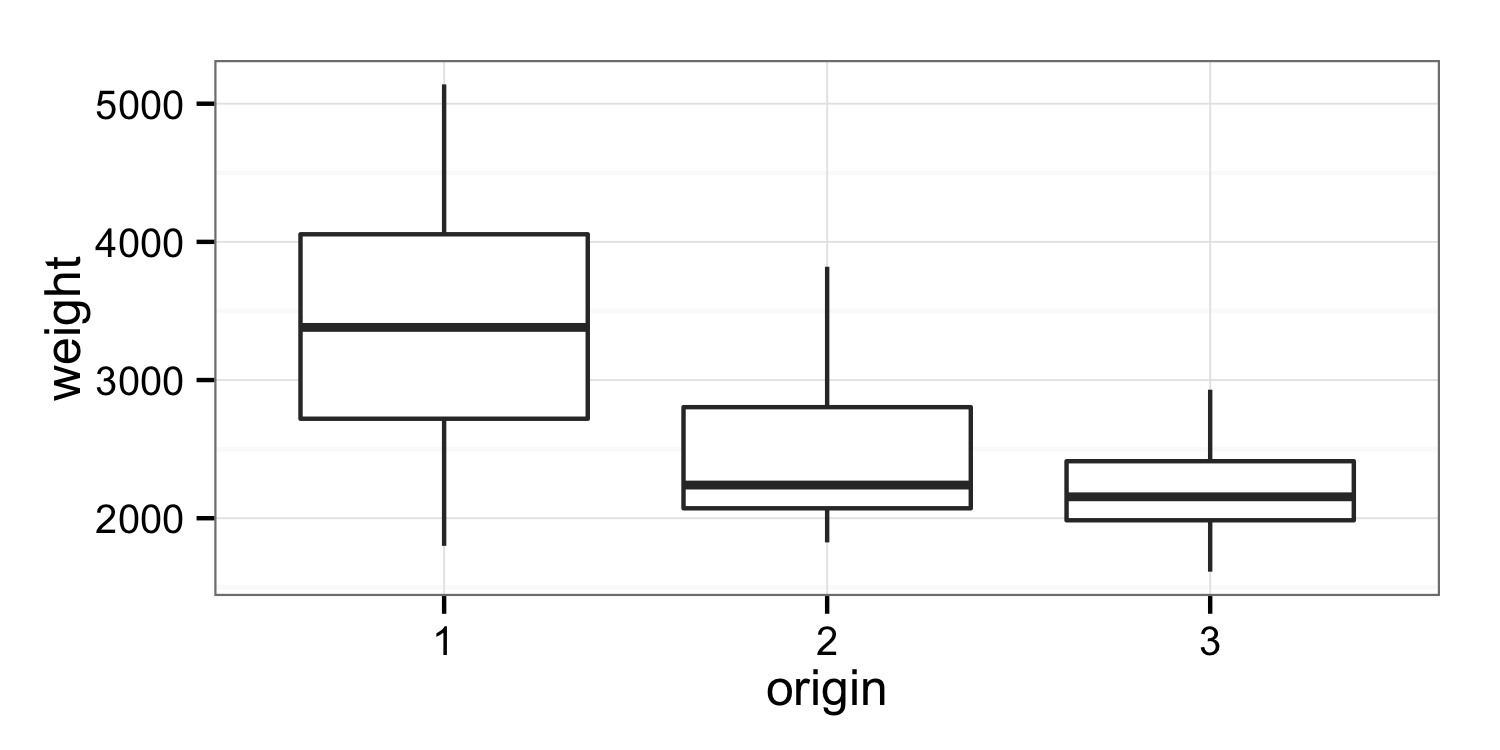
\includegraphics[width=5in]{9e_weight_by_origin.png}
	%\caption{}
	%\label{fig:figName}
\end{figure}


Japanese cars also have higher MPG.
\begin{figure}[H]
	\centering
	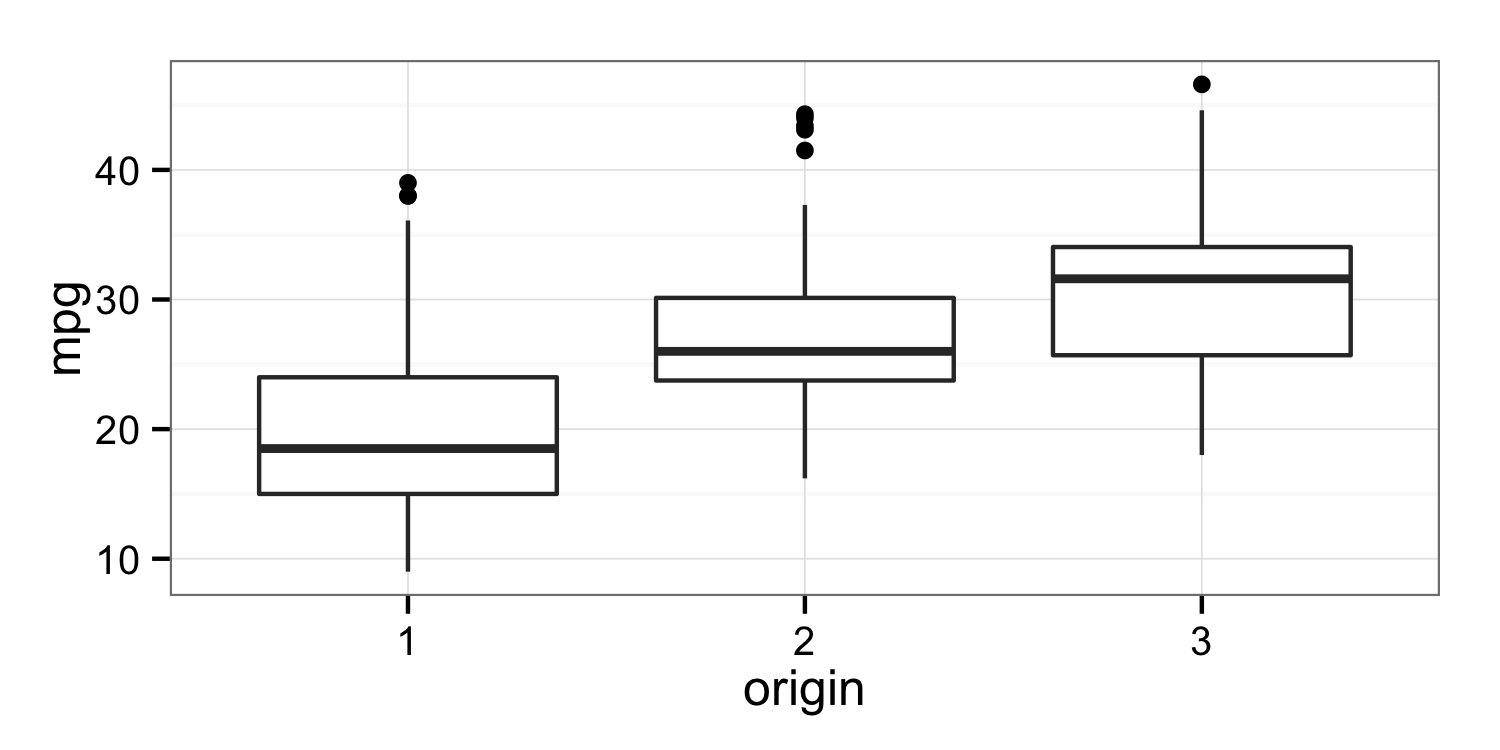
\includegraphics[width=5in]{9e_mpg_by_origin.png}
	\caption{MPG by origin}
	\label{fig:mpg_by_origin}
\end{figure}


\begin{figure}[H]
	\centering
	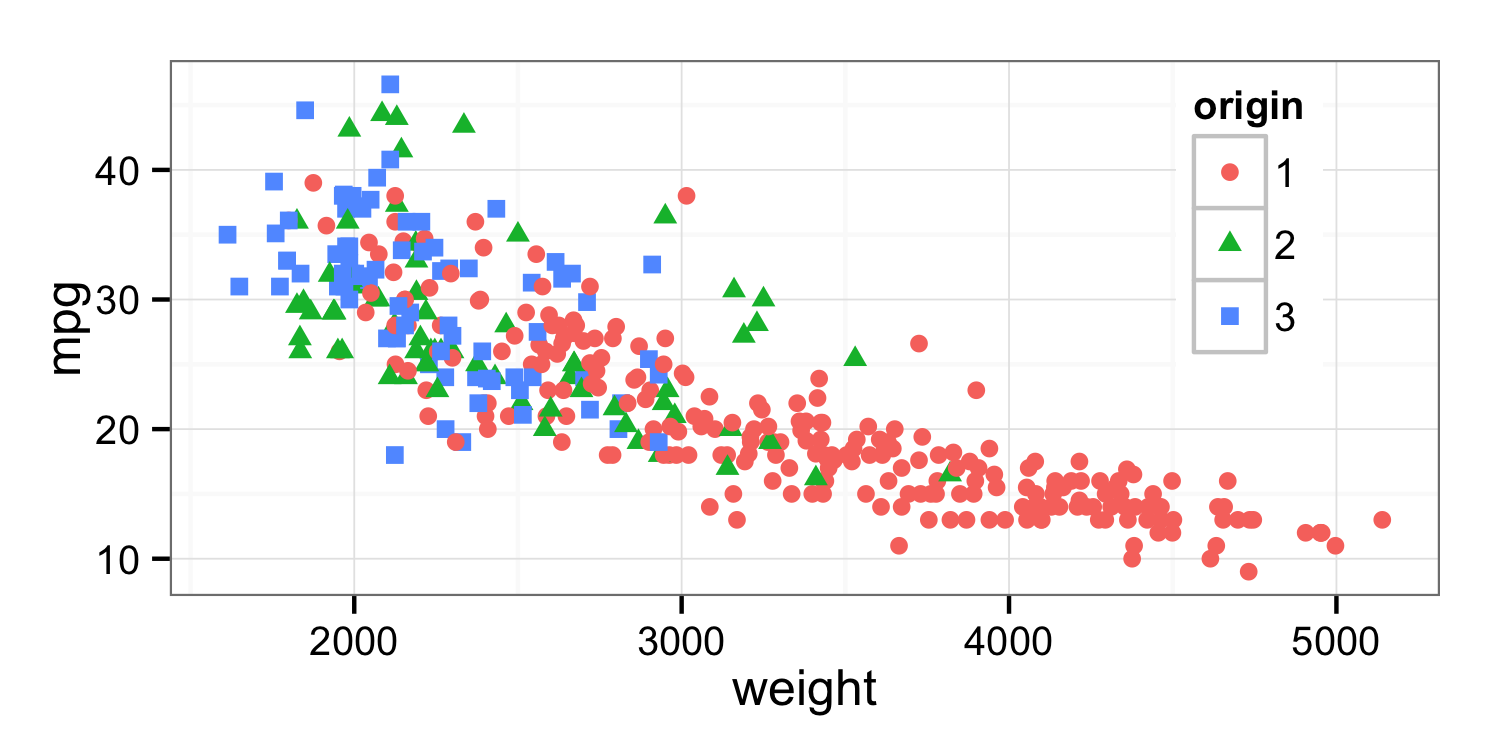
\includegraphics[width=5in]{9e_mpg_vs_weight_by_origin.png}
	\caption{MPG vs weight, by origin}
	\label{fig:mpg_vs_weight_by_origin}
\end{figure}

\subsection*{Part f}

As shown in \textbf{Part e}, the year (Figure \ref{fig:mpg_vs_year}), number of cylinders (Figure \ref{fig:mpg_vs_cyl}), origin (Figure \ref{fig:mpg_by_origin}), and weight (Figure \ref{fig:mpg_vs_weight_by_origin}) of a car are all useful in predicting MPG. Displacement is also a useful predictor, but acceleration is not (see Figures \ref{fig:mpg_by_disp} and \ref{fig:mpg_by_acc} below).

\begin{figure}[H]
	\centering
	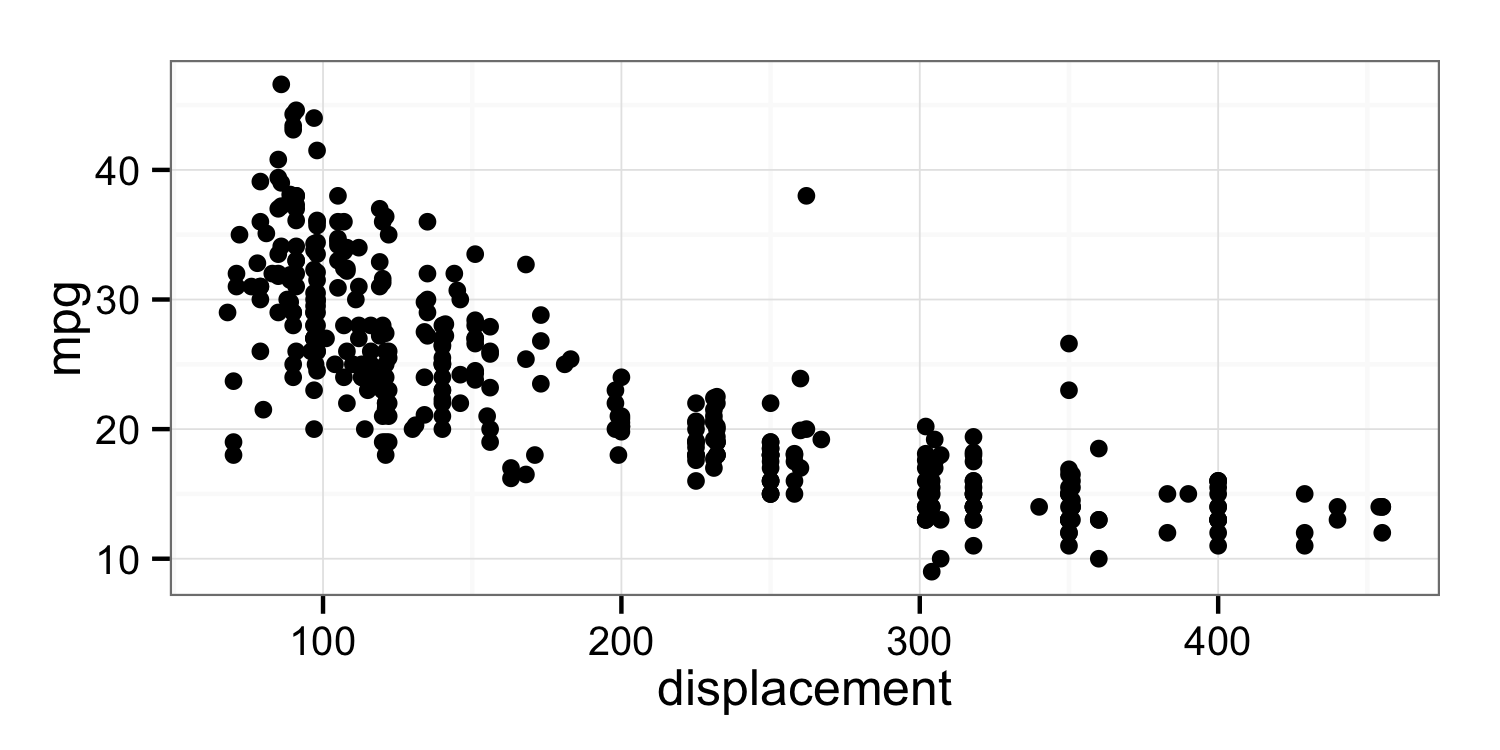
\includegraphics[width=5in]{9e_mpg_vs_disp.png}
	\caption{MPG vs displacemet}
	\label{fig:mpg_by_disp}
\end{figure}

\begin{figure}[H]
	\centering
	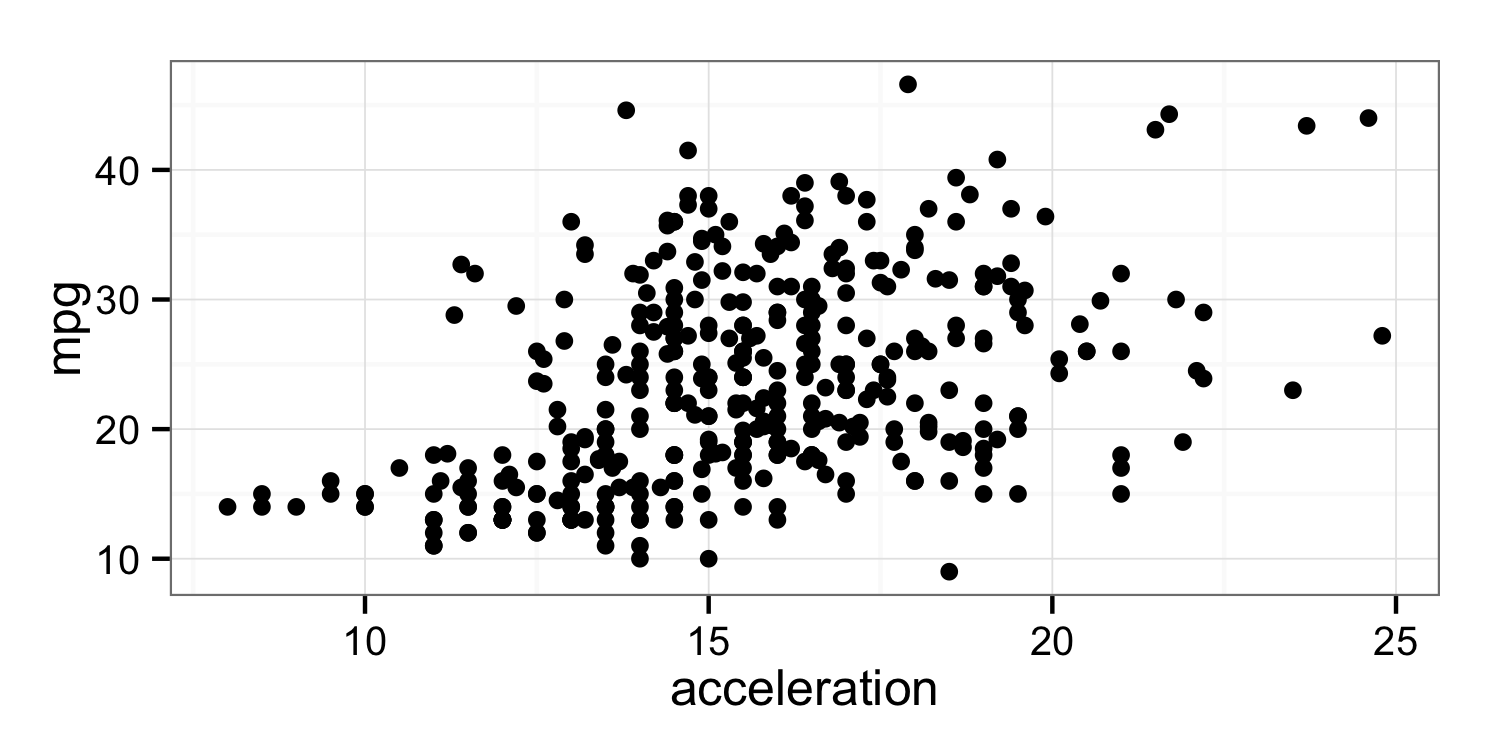
\includegraphics[width=5in]{9e_mpg_vs_acc.png}
	\caption{MPG vs acceleration}
	\label{fig:mpg_by_acc}
\end{figure}



\section*{Problem 3: \href{http://www-bcf.usc.edu/~gareth/ISL/}{James} 2.4, Exercise 10}

\subsection*{Part a}

In the \texttt{Boston} dataset there are 506 rows and 14 columns. Each row represents a town in Boston. The column definitions, as written in the help file, are:
\begin{quote}
\texttt{crim}: per capita crime rate by town.\\
\texttt{zn}: proportion of residential land zoned for lots over 25,000 sq.ft.\\
\texttt{indus}: proportion of non-retail business acres per town.\\
\texttt{chas}: Charles River dummy variable (= 1 if tract bounds river; 0 otherwise).\\
\texttt{nox}: nitrogen oxides concentration (parts per 10 million).\\
\texttt{rm}: average number of rooms per dwelling.\\
\texttt{age}: proportion of owner-occupied units built prior to 1940.\\
\texttt{dis}: weighted mean of distances to five Boston employment centres.\\
\texttt{rad}: index of accessibility to radial highways.\\
\texttt{tax}: full-value property-tax rate per \$10,000.\\
\texttt{ptratio}: pupil-teacher ratio by town.\\
\texttt{black}: $1000(Bk - 0.63)^2$ where Bk is the proportion of blacks by town.\\
\texttt{lstat}: lower status of the population (percent).\\
\texttt{medv}: median value of owner-occupied homes in \$1000s.\\
\end{quote}


\subsection*{Part b}

Pupil-teacher ratio decreases slightly as home value increases.
\begin{figure}[H]
	\centering
	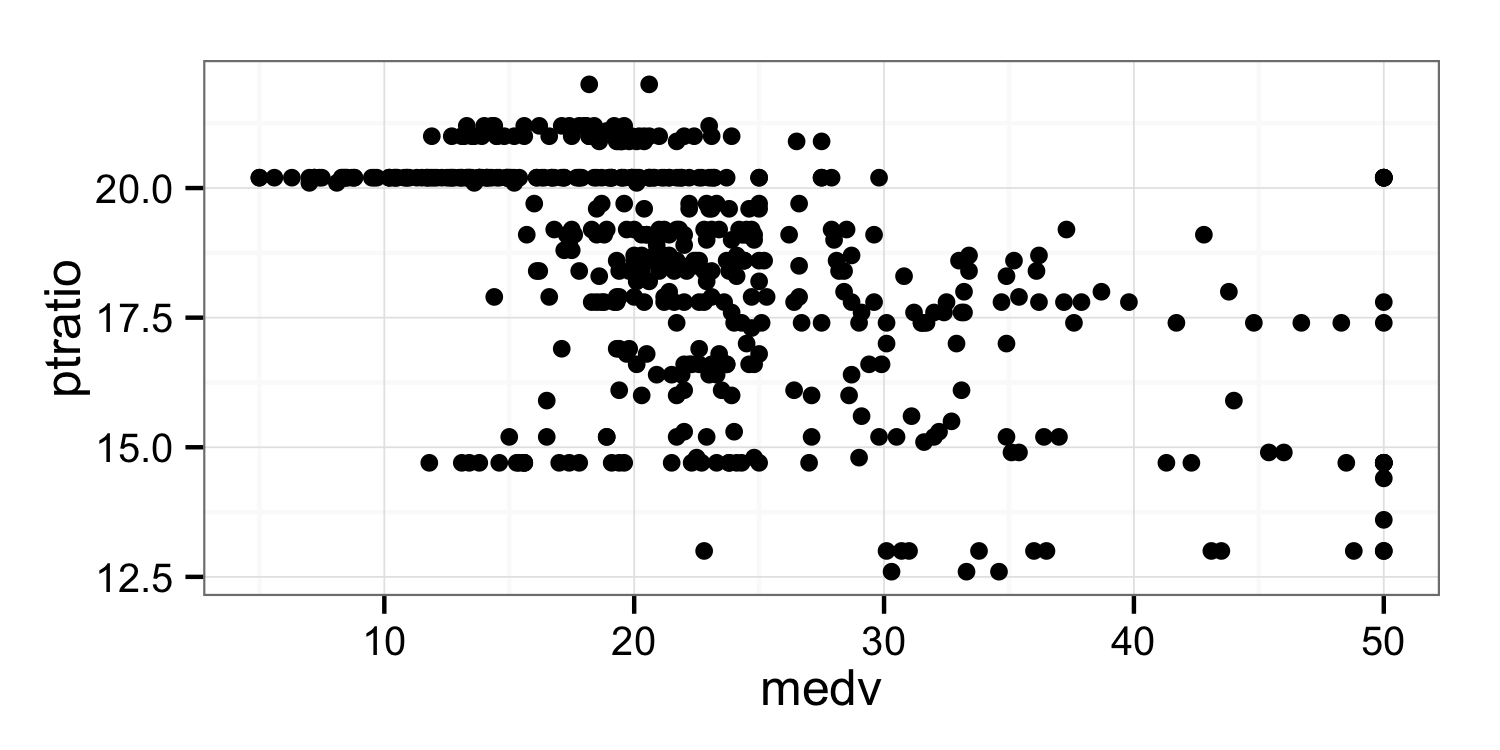
\includegraphics[width=5in]{10b_ptratio_vs_medv.png}
	%\caption{}
	%\label{fig:figName}
\end{figure}

As distance from employment centers increases, nitrogen oxides concentration decreases.
\begin{figure}[H]
	\centering
	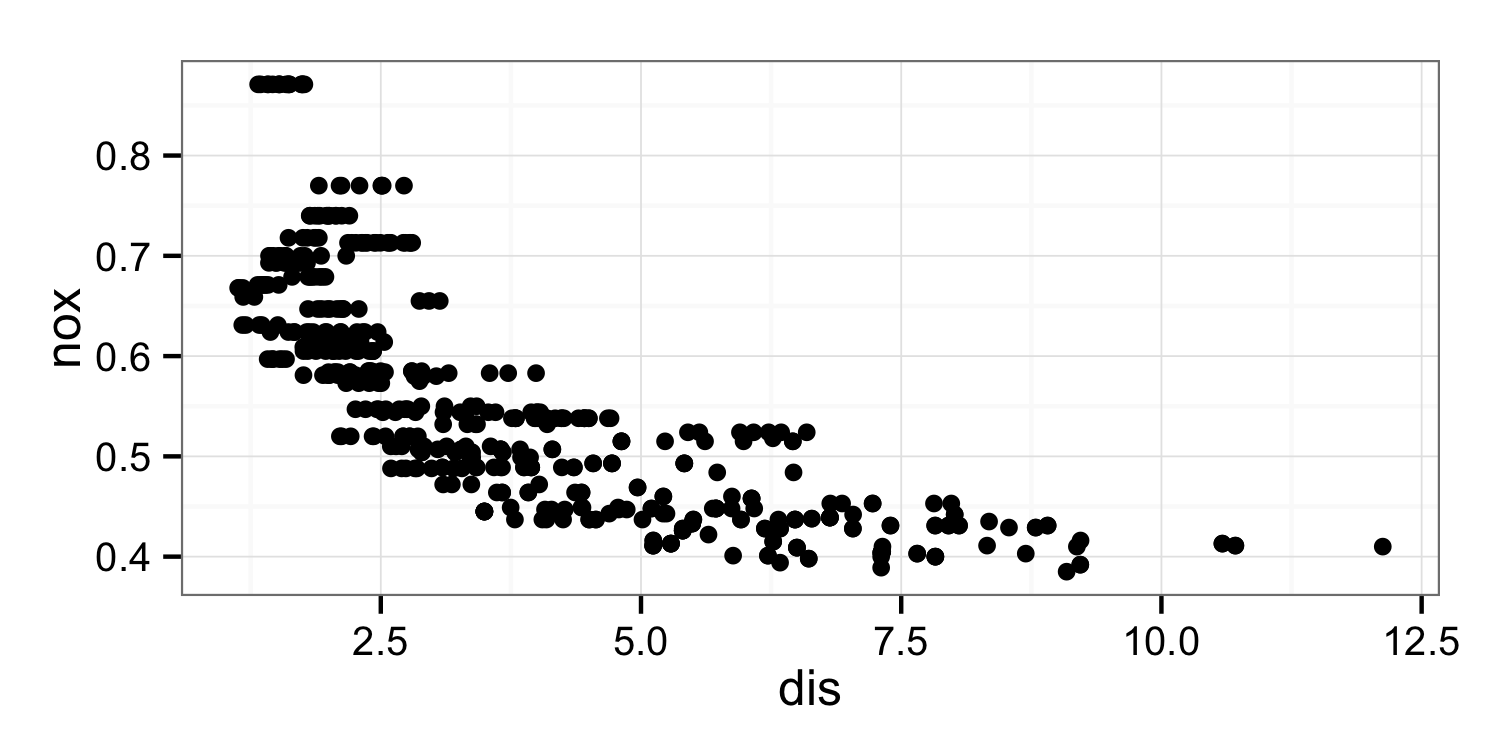
\includegraphics[width=5in]{10b_nox_vs_dis.png}
	%\caption{}
	%\label{fig:figName}
\end{figure}

For plots incorporating crime rate (\texttt{crim}), see \textbf{Part c}.

\subsection*{Part c}

Crime rates are associated with many of the predictors. As "lower status of the population (percent)" increases, crime rates do too.

\begin{figure}[H]
	\centering
	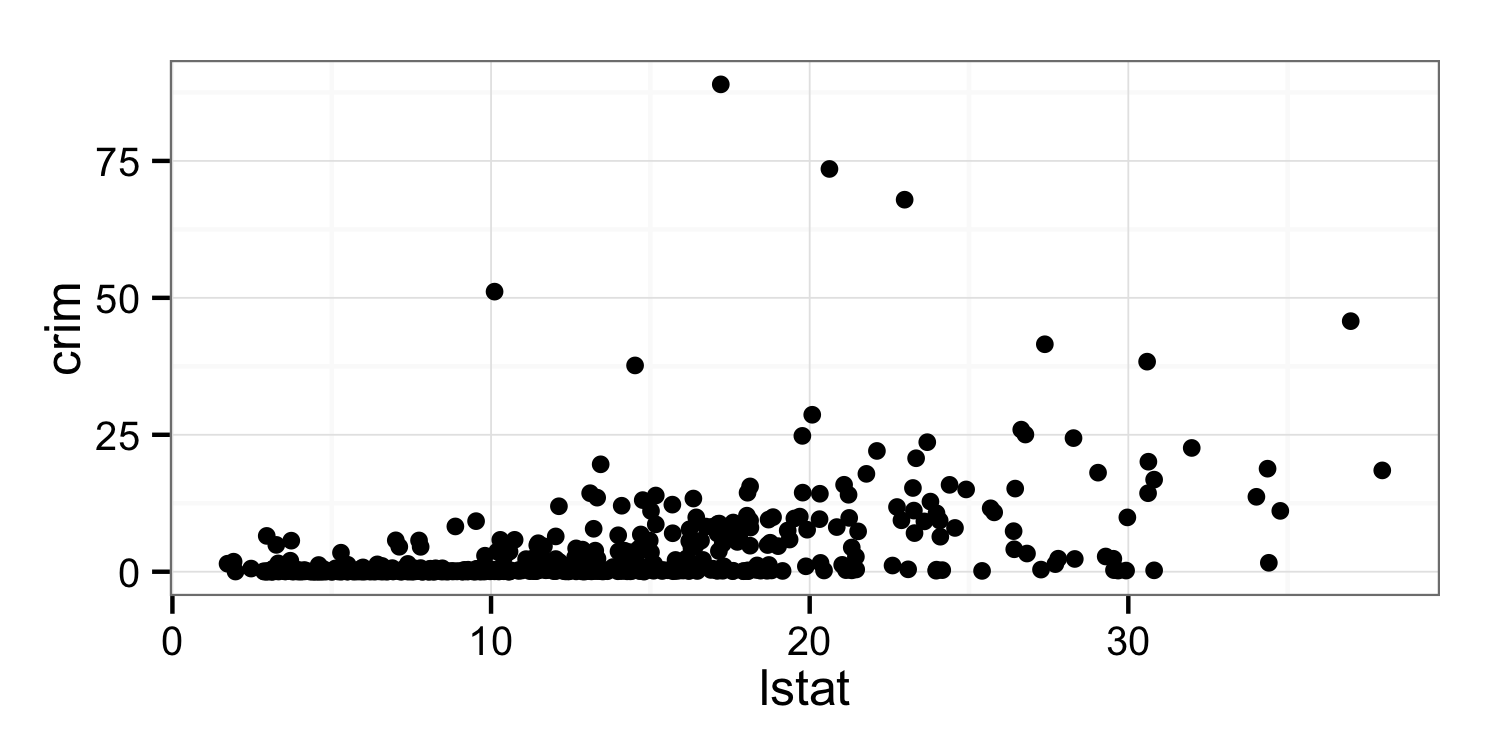
\includegraphics[width=5in]{10b_crim_vs_lstat.png}
	%\caption{}
	%\label{fig:figName}
\end{figure}

Similarly, towns with a higher proportion of buildings built before 1940 have higher crime rates as well.
\begin{figure}[H]
	\centering
	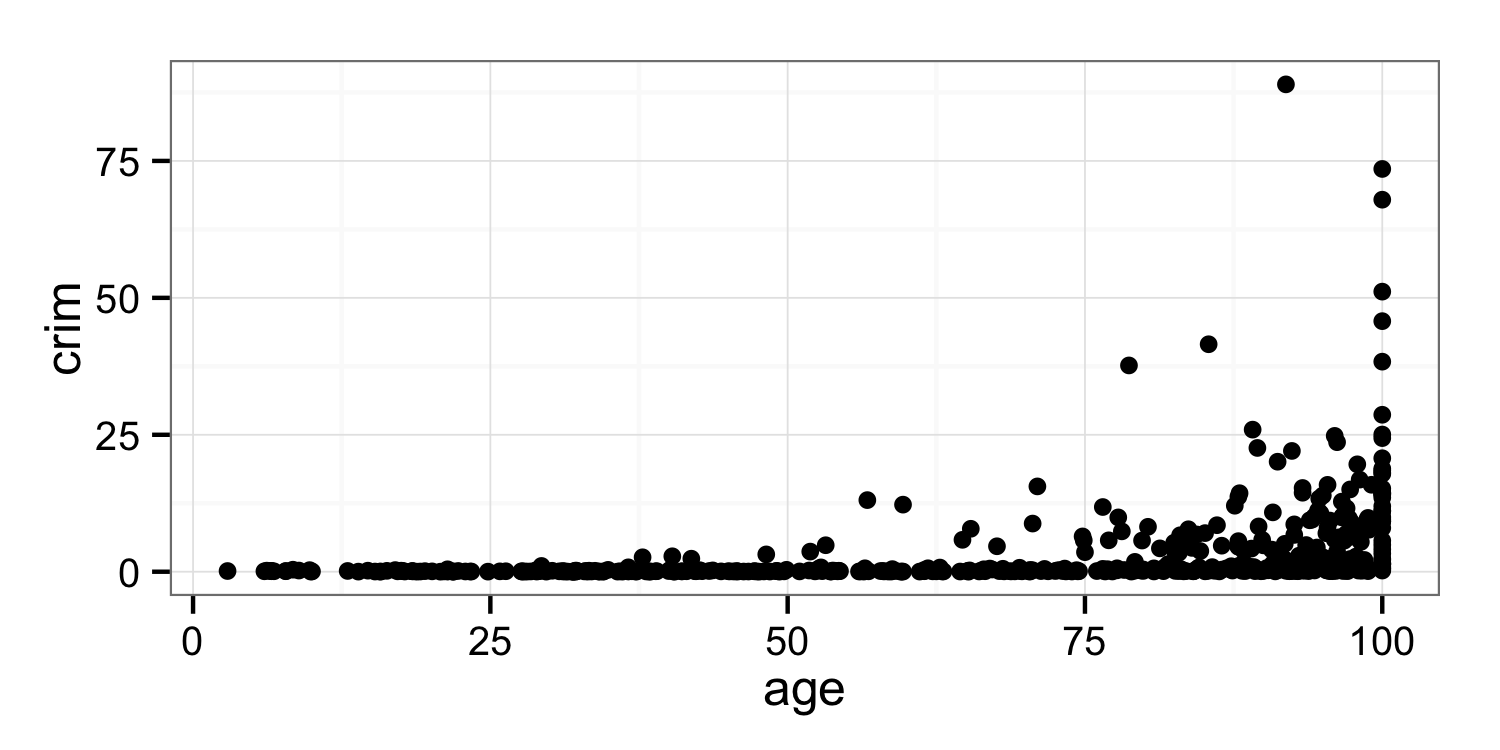
\includegraphics[width=5in]{10b_crim_vs_age.png}
	%\caption{}
	%\label{fig:figName}
\end{figure}

Towns further from employment centers have lower crime rates.
\begin{figure}[H]
	\centering
	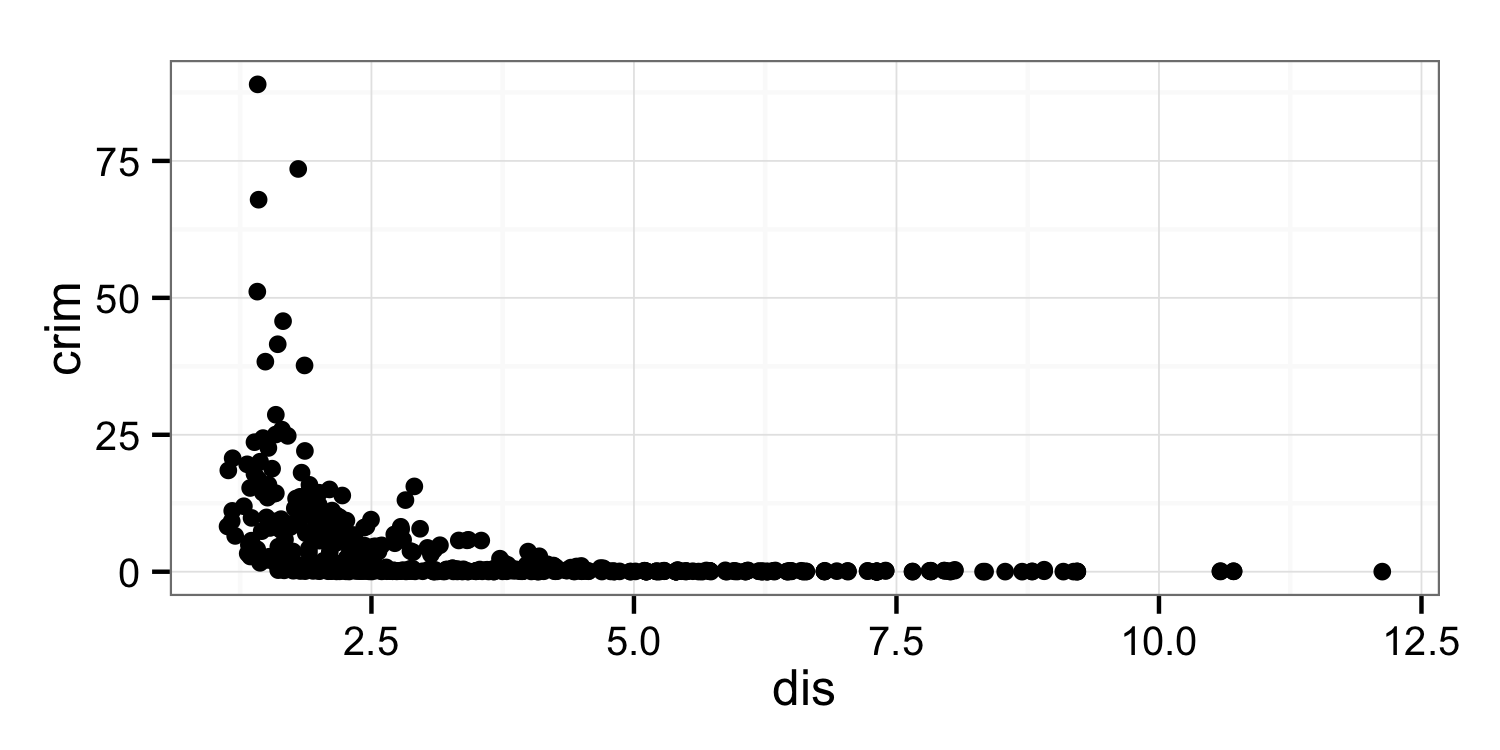
\includegraphics[width=5in]{10b_crim_vs_dis.png}
	%\caption{}
	%\label{fig:figName}
\end{figure}

And crime rates decrease as the median home value increases.
\begin{figure}[H]
	\centering
	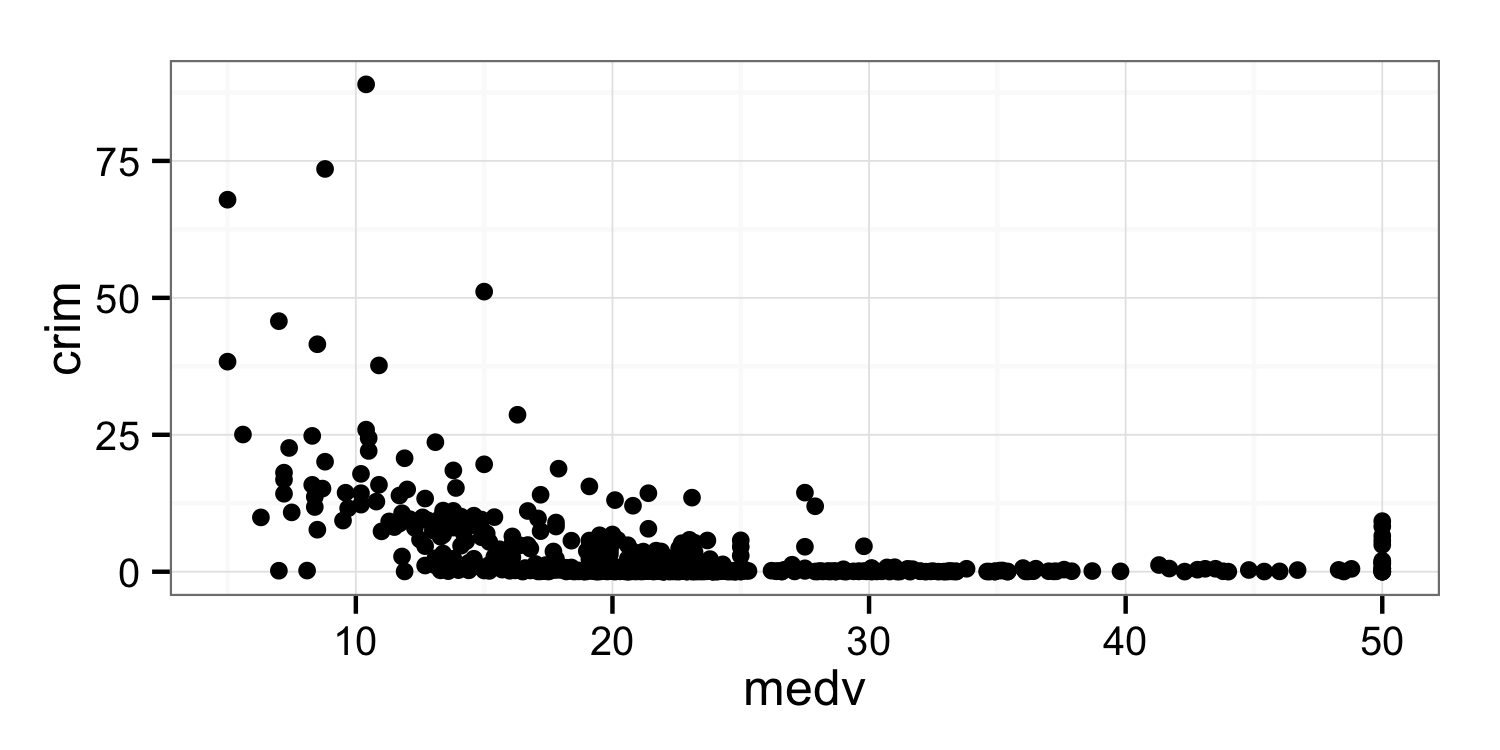
\includegraphics[width=5in]{10b_crim_vs_medv.png}
	%\caption{}
	%\label{fig:figName}
\end{figure}


\subsection*{Part d}


Yes, some suburbs of Bostom appear to have particularly high crime rates. The suburbs in rows 381, 399, 401, 405, 406, 411, 414, 415, 418, 419, and 428 each have a per capita crime rate of more than 25. Crime rate ranges from 0.00632 to 88.97620.\\

There also appear to be some towns with incredibly high tax rates. There are 137 towns with full-value property-tax rate per \$10,000 of more than 600. Tax rate ranges from 187 to 711. A subset of the 137 towns are listed below:
\begin{verbatim}
[1] 357 358 359 360 361 362 363 364 365 366 367 368 369 370 371 372 373
...
[121] 477 478 479 480 481 482 483 484 485 486 487 488 489 490 491 492 493
\end{verbatim}

It doesn't look like any towns have particularly high pupil-teacher ratios. Pupil-teacher ratio ranges from 12.6 to 22.0. 20.2 students/teacher appears to be a very popular ratio.\\


Range of each predictor:
\begin{verbatim}
  stat     crim  zn indus chas   nox    rm   age     dis rad tax ptratio  black lstat medv
1  min  0.00632   0  0.46    0 0.385 3.561   2.9  1.1296   1 187    12.6   0.32  1.73    5
2  max 88.97620 100 27.74    1 0.871 8.780 100.0 12.1265  24 711    22.0 396.90 37.97   50
\end{verbatim}



\subsection*{Part e}

35 town in the dataset bound the Charles river

\subsection*{Part f}

Among towns in the dataset, the median pupil-teacher ratio is 19.05.

\subsection*{Part g}

The towns in row numbers 399 and 406 have the lowest median values of owner-occupied homes at \$5,000.

For those towns:
\begin{verbatim}
  rowNum    crim zn indus chas   nox    rm age    dis rad tax ptratio  black lstat medv
1    399 38.3518  0  18.1    0 0.693 5.453 100 1.4896  24 666    20.2 396.90 30.59    5
2    406 67.9208  0  18.1    0 0.693 5.683 100 1.4254  24 666    20.2 384.97 22.98    5
\end{verbatim}

Crime rates here are on the upper end of the range, and the towns have an average number of rooms per dwelling. Neither town borders the Charles river, and 100\% of owner-occupied buildings in both towns were built before 1940.

\subsection*{Part h}
There are 64 towns that average more than 7 rooms per dwelling, and 13 towns that average more than 8 rooms per dwelling.

Towns with more than 8 rooms per dwelling:
\begin{verbatim}
   rowNum    crim zn indus chas    nox    rm  age    dis rad tax ptratio  black lstat medv
1      98 0.12083  0  2.89    0 0.4450 8.069 76.0 3.4952   2 276    18.0 396.90  4.21 38.7
2     164 1.51902  0 19.58    1 0.6050 8.375 93.9 2.1620   5 403    14.7 388.45  3.32 50.0
3     205 0.02009 95  2.68    0 0.4161 8.034 31.9 5.1180   4 224    14.7 390.55  2.88 50.0
4     225 0.31533  0  6.20    0 0.5040 8.266 78.3 2.8944   8 307    17.4 385.05  4.14 44.8
5     226 0.52693  0  6.20    0 0.5040 8.725 83.0 2.8944   8 307    17.4 382.00  4.63 50.0
6     227 0.38214  0  6.20    0 0.5040 8.040 86.5 3.2157   8 307    17.4 387.38  3.13 37.6
7     233 0.57529  0  6.20    0 0.5070 8.337 73.3 3.8384   8 307    17.4 385.91  2.47 41.7
8     234 0.33147  0  6.20    0 0.5070 8.247 70.4 3.6519   8 307    17.4 378.95  3.95 48.3
9     254 0.36894 22  5.86    0 0.4310 8.259  8.4 8.9067   7 330    19.1 396.90  3.54 42.8
10    258 0.61154 20  3.97    0 0.6470 8.704 86.9 1.8010   5 264    13.0 389.70  5.12 50.0
11    263 0.52014 20  3.97    0 0.6470 8.398 91.5 2.2885   5 264    13.0 386.86  5.91 48.8
12    268 0.57834 20  3.97    0 0.5750 8.297 67.0 2.4216   5 264    13.0 384.54  7.44 50.0
13    365 3.47428  0 18.10    1 0.7180 8.780 82.9 1.9047  24 666    20.2 354.55  5.29 21.9
\end{verbatim}

These towns all have very low crime rates and have lower values for \texttt{lstat}. They generally have \texttt{medv} values towards the higher end of the range.


\section*{Problem 4: Yale Faces B}

\subsection*{Part a}

The $CroppedYale/yaleB01/yaleB01_P00A-005E+10.pgm$ image is of class \texttt{pixmapGrey} (part of the \texttt{pixmap} package). The original image is made up of 32,256 pixels (192 x 168).



\subsection*{Part b}

A pixel value in a \texttt{pixmapGrey}}-classed pgm image ranges from 0 to 1. A value of 0 corresponds to a black pixel, and a value of 1 corresponds to a white pixel.

In \\texttt{faces_matrix}, which combines images 1 and 2, the pixel values range from 0.007843137 to 1.000000000.


\end{document}